% Created 2017-11-13 Mon 11:48
% Intended LaTeX compiler: pdflatex
\documentclass[presentation]{beamer}
\usepackage[utf8]{inputenc}
\usepackage[T1]{fontenc}
\usepackage{graphicx}
\usepackage{grffile}
\usepackage{longtable}
\usepackage{wrapfig}
\usepackage{rotating}
\usepackage[normalem]{ulem}
\usepackage{amsmath}
\usepackage{textcomp}
\usepackage{amssymb}
\usepackage{capt-of}
\usepackage{hyperref}
\usepackage{minted}
\usepackage{helvet}
\usepackage{xcolor}
\definecolor{lgray}{rgb}{0.90,0.90,0.90}
\usetheme{Boadilla}
\usecolortheme{seahorse}
\author{Dale J. Barr}
\date{University of Glasgow}
\title{Advanced Stats: Lec 03 GLMs}
\hypersetup{
 pdfauthor={Dale J. Barr},
 pdftitle={Advanced Stats: Lec 03 GLMs},
 pdfkeywords={},
 pdfsubject={},
 pdfcreator={Emacs 24.5.1 (Org mode 9.0.9)}, 
 pdflang={English}}
\begin{document}

\maketitle

\section*{Logistic regression}
\label{sec:orgf0dc53b}

\begin{frame}[label={sec:orgc7ebca5}]{Continuous vs. discrete data}
Two discrete types of data are common in psychology/linguistics

\begin{itemize}
\item categorical (dichotomous/polychotomous)
\begin{itemize}
\item type of linguistic structure produced (X, Y, Z)
\item region looked at in a visual world study (target, other)
\item number of items recalled out of N
\item accurate or inaccurate selection
\item hired or not hired
\end{itemize}

\item counts (no. opportunities ill-defined)
\begin{itemize}
\item no. of speech errors in a corpus
\item no. of turn shifts in a conversation
\item no. words in a utterance
\end{itemize}
\end{itemize}
\end{frame}

\begin{frame}[label={sec:orgbae2718}]{Why not treat discrete data as continuous?}
\begin{itemize}
\item Proportions range between 0 and 1
\item Variance proportional to the mean (expected probability or rate)
\item Spurious interactions due to scaling effects
\end{itemize}
\end{frame}

\begin{frame}[label={sec:orgfe6b67d}]{Generalized linear models}
\begin{itemize}
\item Allows use of regular linear regression by projecting the DV onto an
appropriate scale

\item Key elements of GLMs: 
\begin{itemize}
\item link function
\item variance function
\end{itemize}
\end{itemize}
\end{frame}

\begin{frame}[label={sec:org9515f98}]{Odds and log odds}
\begin{description}[Bernoulli trial]

\item[Bernoulli trial] An event that has a binary outcome, with one
  outcome typically referred to as ``success''

\item[proportion] A ratio of successes to the total number of
  Bernoulli trials, proportion of days of the week that are Wednesday
  is 1/7 or about .14

\item[odds] A ratio of successes to non-successes, i.e., odds of a
  day being Wednesday are 1 to 6, natural odds= 1/6 = .17

\item[log odds] The (natural) log of the odds (turns multiplicative
  effects into additive effects)

\end{description}
\end{frame}

\begin{frame}[label={sec:org937ac70}]{Properties of log odds or ``logit''}
log odds: \(log\left(\frac{p}{1-p}\right)\) or \(log\left(\frac{Y}{N-Y}\right)\)

where \(p\) is a proportion, \(N\) is total trials and \(Y\) is observed successes

\begin{itemize}
\item Scale goes from \(-\infty\) to \(+\infty\)
\item Scale is symmetric around zero
\item If negative, means that Pr(success)\(<.5\)
\item If positive, Pr(success)\(>.5\)
\end{itemize}
\end{frame}

\begin{frame}[label={sec:org0275250}]{Logistic regression}
\begin{columns}[T]
\begin{column}{.5\textwidth}
DV has 2 categories\\[6pt]
\structure{model}\\
$\eta = \beta_0 + \beta_1 X$\\
\vspace{6pt}
\structure{link function}\\
$\eta = log\left(\frac{p}{1-p}\right)$\\
\vspace{6pt}
\structure{inverse link function}\\
$p = \frac{1}{1+exp(-\eta)}$\\
getting odds from logit: exp($\eta$)\\
\vspace{6pt}
\structure{variance function} (binomial)\\
$np(1-p)$\\
\end{column}
\begin{column}{.5\textwidth}
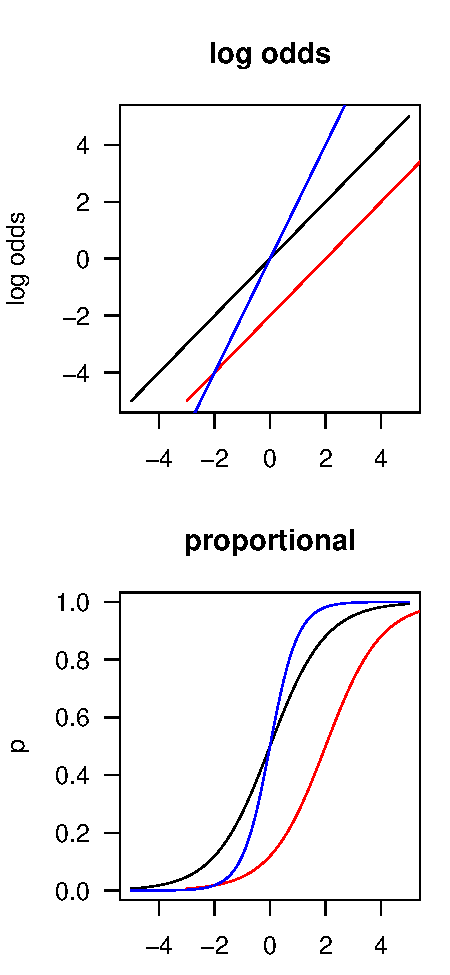
\includegraphics[scale=.4]{img/logit}
\end{column}
\end{columns}
\end{frame}

\section*{Titanic dataset}
\label{sec:org957467c}

\begin{frame}[fragile,label={sec:orgbe7c938}]{Titanic dataset (kaggle)}
 \begin{columns}
\begin{column}{.37\columnwidth}
\begin{tiny}

\begin{verbatim}
VARIABLE DESCRIPTIONS:
survival        Survival
                (0 = No; 1 = Yes)
pclass          Passenger Class
                (1st; 2nd; 3rd)
name            Name
sex             Sex
age             Age
sibsp           N Siblings/Spouses Aboard
parch           N Parents/Children Aboard
ticket          Ticket Number
fare            Passenger Fare
cabin           Cabin
embarked        Port of Embarkation
                (C = Cherbourg; 
                 Q = Queenstown; 
                 S = Southampton)
\end{verbatim}

\end{tiny}
\end{column}

\begin{column}{.63\columnwidth}
\begin{tiny}

\begin{verbatim}
SPECIAL NOTES:
Pclass is a proxy for socio-economic status (SES)
 1st ~ Upper; 2nd ~ Middle; 3rd ~ Lower

Age is in Years; Fractional if Age less than One (1)
 If the Age is Estimated, it is in the form xx.5

With respect to the family relation variables (i.e. sibsp and parch)
some relations were ignored.  The following are the definitions used
for sibsp and parch.

Sibling:  Brother, Sister, Stepbrother, or Stepsister of Passenger 
           Aboard Titanic
Spouse:   Husband or Wife of Passenger Aboard Titanic 
           (Mistresses and Fiances Ignored)
Parent:   Mother or Father of Passenger Aboard Titanic
Child:    Son, Daughter, Stepson, or Stepdaughter of Passenger 
           Aboard Titanic

Other family relatives excluded from this study include cousins,
nephews/nieces, aunts/uncles, and in-laws.  Some children travelled
only with a nanny, therefore parch=0 for them.  As well, some
travelled with very close friends or neighbors in a village, however,
the definitions do not support such relations.
\end{verbatim}

\end{tiny}
\end{column}
\end{columns}
\end{frame}



\section*{Logit models}
\label{sec:org9e628b0}
\end{document}
